\documentclass[letterpaper,12pt]{article}
\usepackage{courier}
\usepackage{fancyheadings}
\usepackage{verbatim}
\usepackage{hyperref}
\usepackage{graphicx}
\pagestyle{fancy}
\setlength\textwidth{6.5in}
\setlength\textheight{8.5in}
\newtheorem{problem_statement}{Problem Statement}
\newcommand{\TBC}{\framebox{\textbf{TO BE COMPLETED}}}
\newtheorem{assumption}{Assumption}
\newcommand{\be}{\begin{enumerate}}
\newcommand{\ee}{\end{enumerate}}
\newcommand{\bi}{\begin{itemize}}
\newcommand{\ei}{\end{itemize}}
\newtheorem{notation}{Notation}
\newtheorem{definition}{Definition}
\newcommand{\ReportDate}{Jan 1, 2023}
\newcommand{\NumDataSets}{__NumDataSets__}
\newcommand{\NumFormulas}{5}
\newcommand{\MinNumRows}{__min_num_rows_read__}
\newcommand{\MaxNumRows}{__max_num_rows_read__}
\newcommand{\AvgNumRows}{__avg_num_rows_read__}


\newcommand{\NumPLPSuccessA}{__NumPLPSuccessA__}
\newcommand{\NumPLPErrorsA}{__NumPLPErrorsA__}
\newcommand{\AvgTimePLPA}{__AvgTimePLPA__}

\newcommand{\NumPLPErrorsB}{__NumPLPErrorsB__}
\newcommand{\NumPLPAttemptsB}{__NumPLPAttemptsB__}
\newcommand{\AvgTimePLPB}{__AvgTimePLPB__}

\newcommand{\NumDataSetsForModel}{X}
\newcommand{\NumModelsAttempted}{X}
\newcommand{\NumModelsSucceeded}{X}
\newcommand{\ModelMinTime}{X}
\newcommand{\ModelMaxTime}{X}
\newcommand{\ModelAvgTime}{X}

\begin{document}
\title{Overview of DFE Run}
\author{Automated}
\maketitle
\thispagestyle{fancy}
\lhead{}
\chead{}
\rhead{}
% \lfoot{{\small Decision Sciences Team}}
\cfoot{}
\rfoot{{\small \thepage}}

\begin{abstract}
\ This is an automatically generated report. It is meant ot illustrate the kinds
of analysis that can be performed in LightR.
\end{abstract}

\section{Overview}

\bi
\item The report was generated on \ReportDate. 
\item The number of data sets was \NumDataSets.
\item Summary statistics of number of rows in data set:
  \bi
\item Minimum \MinNumRows
\item Maximum \MaxNumRows
\item Average \AvgNumRows
  \ei
\item The number of formulas per model was \NumFormulas.
  Explanation of the formulas is in Table~\ref{tbl_formulas}.
  \ei

\section{Basic Feature Engineering}
\label{PLP1}
\bi
\item The number of times this was invoked was \NumDataSets
\item The number of errors reported was \NumPLPErrorsA.
\item The average time taken (in \(\mu\,\)seconds) was \AvgTimePLPA
\ei

Distribution of occurrence of error codes is shown in Table~\ref{plp1_errs}

Explanation of error codes is in Table~\ref{explanation_plp1_errs}
\begin{table}
  \centering
  \begin{tabular}{|l|l|} \hline \hline
    {\bf Error Code} & {\bf Count} \\ \hline 
    \input{plp1_error_count.csv} 
    \hline
  \end{tabular}
  \caption{Error Counts for basic feature engineering}
  \label{plp1_errs}
\end{table}

\section{Formula Specific Feature Engineering}
\label{PLP2}

\bi
\item The number of times this was invoked was \NumPLPAttemptsB.
\item The number of data sets that had at least one error was
  \NumPLPErrorsB.
\item The average time taken (in \(\mu\,\)seconds) was \AvgTimePLPB
\ei

Distribution of occurrence of error codes (by formula) is shown in Table~\ref{plp2_errs}

Explanation of error codes is in Table~\ref{explanation_plp2_errs}
\begin{table}
  \centering
  \begin{tabular}{|l|l|l|} \hline \hline
    {\bf Formula} & {\bf Attempts} & {\bf Successes} \\ \hline 
    \input{plp2_error_count.csv} 
    \hline
  \end{tabular}
  \caption{Error Counts for formula specific feature engineering}
  \label{plp2_errs}
\end{table}

Distribution of errors by formula and type is shown in Table~\ref{plp2_errs_B}
\begin{table}
  \centering
  \begin{tabular}{|l|l|l|} \hline \hline
    {\bf Formula} & {\bf Error Code} & {\bf Count} \\ \hline 
    \input{plp2_error_countB.csv}  
    \hline
  \end{tabular}
  \caption{Error Counts, broken down by formula and type}
  \label{plp2_errs_B}
\end{table}

\section{Model Building}
\bi
\item The number of data sets for which model building was attempted was
  \NumDataSetsForModel
\item The number of models attempted was \NumModelsAttempted
\item The number of models that were built was \NumModelsSucceeded
\item Summary statistics of time (in seconds) to build a model
  \bi
\item Minimum \ModelMinTime
\item Maximum \ModelMaxTime
\item Average \ModelAvgTime
\ei
\item Distribution of build times is in Figure~\ref{fig_model_build_times}
\ei
\begin{figure}
\fbox{
  \begin{minipage}{6.0in}
  \centering
  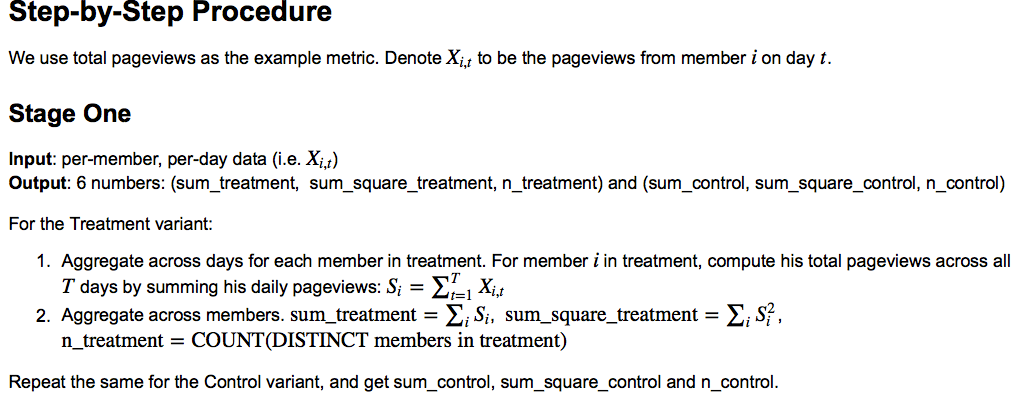
\includegraphics[width=4.5in]{model_build_times.png}
    \caption{Distribution of model build times (seconds)}
  \label{fig_model_build_times}
  \end{minipage}
}
\end{figure}

\section{Explanations of Terms}
\subsection{Formulas}

\begin{table}
  \centering
  \begin{tabular}{|l|l|l|} \hline \hline
    {\bf Index} & {\bf Key} {\bf Explanation} \\ \hline 
     % Make sure exactly one line per valid formula
 0 & f0 & Basic formulas \\ \hline
 1 & f1 & Uses 2 lag components (week 1 and week 2) \\ \hline
 2 & f2 & Uses 2 lag components (week 2 and week 3) \\ \hline
 3 & f3 & Uses 2 lag components (week 3 and week 4) \\ \hline
 4 & f4 & Uses 2 lag components (week 4 and week 5) \\ \hline
 
    \hline
  \end{tabular}
  \caption{List of Formulas}
  \label{tbl_formulas}
\end{table}

\section{Error Codes}

\subsection{Basic Feature Engineering}
See Table~\ref{explanation_plp1_errs}
\begin{table}
  \centering
  \begin{tabular}{|l|l|} \hline \hline
    {\bf Error Code} & {\bf Explanation} \\ \hline  \hline
     % Make sure exactly one line per valid error code value
    0 & No Error \\ \hline 
    1 &  insufficient rows in input data frame  \\ \hline
    2 &  insufficient rows in input data frame after cleaning \\ \hline
    3 &  insufficient unique values in {\bf toy} component \\\hline

    \hline
  \end{tabular}
  \label{explanation_plp1_errs}
  \caption{Explanation of Error Codes}
\end{table}

\subsection{Formula Specific Feature Engineering}

See Table~\ref{explanation_plp2_errs}
\begin{table}
  \centering
  \begin{tabular}{|l|l|} \hline \hline
    {\bf Error Code} & {\bf Explanation} \\ \hline  \hline
     % Make sure exactly one line per valid error code value
    0 & No Error \\ \hline 
    1 &  not enough rows after cleaning  \\ \hline
    2 &  Range of {\bf toy} component too small \\ \hline
    3 &   too few uniques  in {\bf toy} component \\ \hline
    4 &  too few uniques in lag component \\ \hline

    \hline
  \end{tabular}
  \label{explanation_plp2_errs}
  \caption{Explanation of Error Codes}
\end{table}

\end{document}

